\newpage

\section{Sprint 2} 

Il progetto di riferimento per questo sprint è it.unibo.ddrSystem2.

\textbf{OBIETTIVO}: creazione di un robot in grado di esplorare una stanza rettangolare vuota. Il robot, durante l'esplorazione della stanza, dovrà essere in grado di costruire incrementalmente una mappa della stanza.

\subsection{Work Plan}

\begin{enumerate}
    \item utilizzare il simulatore di Soffritti (robot virtuale) per verificare che il sistema creato funzioni correttamente. Nell'effettuare il collegamento tra i due si rimarrà technology independent (robotSupport);
    
    \item utilizzare un robot fisico (realnano) per verificare che il sistema creato funzioni correttamente e che la scelta tecnologica non impatti sull'architettura logica del sistema. Il robot deve essere in grado di muoversi in avanti, in indietro, ruotare a destra, a sinistra e fermarsi, proprio come quello simulato;
    
    \item definizione della strategia di esplorazione della stanza.
    
    \item progettazione del test plan per verificare che il robot riesca a costruire correttamente la mappa della stanza seguendo la strategia scelta.
       
    \item progettazione di una strategia per la creazione della mappa relativa alla stanza. Valutare le diverse possibilità: utilizzo di una base di conoscenza prolog, creazione di una libreria per la gestione della mappa, utilizzo di plannerUtils già fornite. 
 
\end{enumerate}{}


\subsection{Analisi dei requisiti}

\textbf{Cosa si intende per esplorazione della stanza?}\\
Per esplorazione si intende muovere il robot in maniera organizzata e autonoma dentro ad una stanza finché non sono state esplorate tutte le celle. Ad esempio, un risultato che si potrebbe ottenere a fine esplorazione è il seguente:\newline   
r, 1, X,\\
1, 1, X,\\
X, X, X\\

\textbf{Quali informazioni raccoglierà in fase di esplorazione?}\\
Il robot raccoglie le informazioni riguardanti la stanza, in particolare, quali celle sono state visitate, quali ancora no e dove si trovano i muri.

\textbf{Quando il robot inizia ad esplorare autonomamente la stanza?}\\
Quando riceve il comando di "start" (R-startExplore) dalla console.

\textbf{Quando il robot smette di esplorare autonomamente la stanza?}\\
Quando riceve il comando di "stop" (R-stopExplore) dalla console.


\subsection{Analisi del problema}


Esistono varie strategie per permettere al robot di raggiungere l'obiettivo, ognuna di queste prevede che la posizione iniziale (base) del robot coincida con uno degli angoli della stanza e che la distanza percorsa dal robot ad ogni spostamento sia unitaria (in questo caso, l'unità di riferimento è la dimensione del robot). Le strategie vagliate sono le seguenti:
\begin{itemize}
    \item \textbf{a chiocciola}: utilizzando questa strategia il robot esplora in maniera incrementale tutta la superficie della stanza, inizialmente il robot percorre la parte di stanza a lui strettamente adiacente per poi, a mano a mano, espandersi sino ad esplorarla per intero.
    
    \item \textbf{a colonne/righe}: utilizzando questa strategia il robot esplora la stanza muovendosi inizialmente lungo un lato finché non incontra il muro opposto. Una volta incontrato si gira di $90^\circ$ nella direzione in cui non sono presenti muri. Poi si sposta di una unità, si rigira di  $90^\circ$ e procede dritto fino a che non rincontra un altro muro. 
    Al termine dell'esecuzione il robot si deve trovare o nell'angolo opposto (nel caso in cui il numero di colonne/righe fosse dispari) oppure nell'angolo adiacente (nel caso in cui il numero di colonne/righe fosse pari).
    Il modo per implementare questa strategia potrebbe essere quello di creare un robot che percorra tutta la lunghezza di un solo lato della stanza.
    
    \item \textbf{a spirale}: utilizzando questa strategia il robot si muove dapprima lungo le quattro pareti (in maniera oraria e sempre lungo la parente adiacente successiva rispetto a quella che è appena stata esaminata), dopodiché effettua il medesimo tragitto ma restringendo il campo da esplorare. L'esplorazione procede per rettangoli concentrici via via sempre più piccoli e termina quando il robot si trova nel centro della stanza.
\end{itemize}

Esistendo diverse strategie per realizzare questo compito si può pensare di incapsulare la logica di comportamento in più componenti esterni per poi utilizzare quello desiderato.


\subsection{Model}
Si è scelta la strategia della chiocciola per l'esplorazione autonoma in quanto si ritiene che essa sia quella che ottimizza il ritrovamento della bomba, poiché permette di effettuare una ricerca più omogenea e quindi di ritrovare la bomba as soon as possible.
Dato che si ritiene importante dividere la logica di esplorazione del robot dall'attuazione di essa, partendo dal QActor \texttt{robot} modellato nello sprint precedente, si è deciso di suddividerlo in due QActor differenti, ossia:
\begin{itemize}
    \item \texttt{robotmind}: ha il compito di pianificare le azioni necessarie per raggiungere una determinata posizione sulla mappa (vedi funzione \texttt{setGoal(X,Y)}); posizione che diventerà incrementalmente sempre più lontana dalla quella iniziale in quanto si è scelto di esplorare la stanza con la strategia della chiocciola e la cui massima distanza dalla base coinciderà con l'angolo opposto della stanza. Una volta pianificate le azioni per raggiungere un punto della stanza, queste verranno eseguite una alla volta e, in presenza di un ostacolo (muro), una delle azioni fallirà e comporterà il ricalcolo del tragitto che il robot dovrà percorrere (\texttt{vedi State setGoalAfterWall}). 
    
    Il codice di robotmind è riportato nel Listing \ref{lst:robotmind_ddr_sys_2}.
    \item \texttt{robotactuator}: ha il compito di eseguire una alla volta le azioni (vedi \texttt{move(msg(M))} pianificate da \texttt{robotmind}. 
    
    Il codice di robotactuator è riportato nel Listing \ref{lst:robotactuator_ddr_sys_2}.

\end{itemize}
Analizzando i movimenti del robot si è evidenziato che il robot può incontrare un muro solamente quando si muove in avanti, dunque si è introdotto un terzo QActor: \texttt{onestepahead}. In particolare, questo attore riceverà un messaggio \texttt{onestep} (vedi funzione \texttt{attemptToMoveAhead()}) che farà muovere il robot in avanti e controllerà se effettivamente il movimento è possibile. Se il movimento è possibile, in quanto non vi sono ostacoli, ciò verrà notificato a \texttt{robotmind} con un messaggio di \texttt{stepOk} altrimenti \texttt{robotmind} riceverà un messaggio di \texttt{stepFail}.
Il codice di onestepahead è riportato nel Listing \ref{lst:onestepahead_ddr_sys_2}.

L'architettura del sistema è riportata in \cref{fig:sprint2_logic}

\begin{figure} [H]
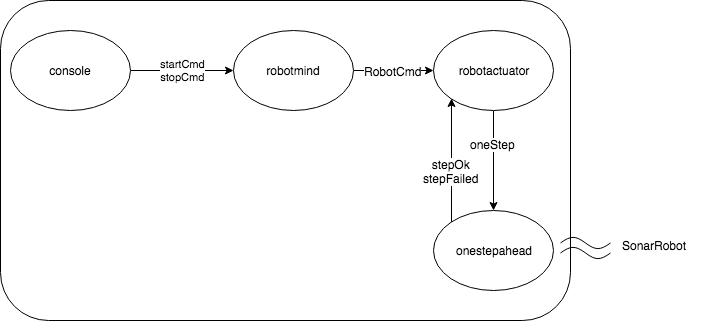
\includegraphics[width=\linewidth]{img/sprint2/sprint2_logic.png}
\caption{Architettura logica del sistema dello sprint 2.}
\label{fig:sprint2_logic}
\end{figure}



\begin{lstlisting}[backgroundcolor=\color{white}, label={lst:robotmind_ddr_sys_2}, caption={Codice di QActor robotmind in ddrSystem2} ]

QActor robotmind context ctx { 
["var Curmove     = \"\"  
var IterCounter = 0 
var backHome = false
var maxX = 0
var maxY = 0
var finish = false

//VIRTUAL ROBOT
var StepTime   = 330	 
 
var Tback       = 0
"]
	State s0 initial {
		println("&&&  robotmind STARTED")
		solve (consult ("ddrsys.pl")) 
		solve (consult ("resourceModel.pl")) 
		println("Robot intialized")
		run itunibo.planner.plannerUtil.initAI()
		println("INITIAL MAP") 
		run itunibo.planner.plannerUtil.showMap() 
		
	} 
	
	Goto waitForStart
	
	State waitForStart {	printCurrentMessage }
	
	Transition t0  whenMsg startCmd  -> startExploration
				   whenMsg startTest -> startExplorationTest
	
	State startExplorationTest {
		["finish = true
		  backHome = false

		  var x = \"\"
		  var y = \"\"	"]
		println("&&&  exploration TEST")
		
		printCurrentMessage		        
 		onMsg( startTest : startTest(X, Y) ) { 
 			[" x =payloadArg(0) 
			   y =payloadArg(1) "]
		run itunibo.planner.plannerUtil.setGoal(x,y)
		run itunibo.planner.moveUtils.doPlan( myself ) //moves stored in actor kb	
 		}
	}
	Goto doPlan
	
	
	State startExploration {
		println("&&&  exploration STARTED")
		run itunibo.planner.plannerUtil.setGoal("1","1")
		run itunibo.planner.moveUtils.doPlan( myself ) //moves stored in actor kb
	}
	
	Goto doPlan
	
	//raggiungo la cella
	State doPlan {	
		run itunibo.planner.plannerUtil.showMap() 
		solve( retract( move(M) ) ) 	//consume a move
		ifSolved {  ["Curmove = getCurSol(\"M\").toString()"]  }
		 else { ["Curmove=\"nomove\" "]  }
	}  
	
	Goto handlemove if "(Curmove != \"nomove\")" else choose
	
	State handlemove {}
	
	Goto domove if "(Curmove != \"w\")" else attempttogoahead
	
	State domove {
		run itunibo.planner.moveUtils.doPlannedMove(myself, Curmove)
		forward robotactuator -m robotCmd : robotCmd(\$Curmove)
		delay 700
		forward robotactuator -m robotCmd : robotCmd(h)
	}
	
	Goto doPlan
	
	//roomboundaryplanning.qak
	State attempttogoahead {	
		run itunibo.planner.moveUtils.attemptTomoveAhead(myself, StepTime)
	}
	Transition t0   whenMsg stepOk   -> stepDone   
					whenMsg stepFail -> stepFailed 
	 
 	State stepDone{  
 		run itunibo.planner.moveUtils.doPlannedMove(myself, "w")	
 	}
 	
 	Goto doPlan
 	
 	State stepFailed{
 		println("&&&  FOUND WALL")
["var TbackLong = 0L"]		 
 	  	
		//printCurrentMessage		        
 		onMsg( stepFail : stepFail(Obs, Time) ) { 
 			["Tback=payloadArg(1).toLong().toString().toInt() / 2
			TbackLong = Tback.toLong()"]
 			println("stepFailed \${payloadArg(1).toString()}")
 		}
  		
 		println(" backToCompensate stepTime=\$Tback")
 		forward robotactuator -m robotCmd : robotCmd(s)
		delayVar TbackLong
		forward robotactuator -m robotCmd : robotCmd(h)
		delay 700
 //--------------------------------------------------
 		run itunibo.planner.plannerUtil.wallFound()
 	
	}   
	
	//Goto endOfJob //**checkWallTest
	Goto setGoalAfterWall
	
	State setGoalAfterWall{
		solve( retractall( move(_) ))
	["
	if( itunibo.planner.plannerUtil.getDirection() == \"downDir\" ){ 
		maxY = itunibo.planner.plannerUtil.getPosY()
		if(maxX == 0 ){
			itunibo.planner.plannerUtil.setGoal(IterCounter, maxY)
		} else {itunibo.planner.plannerUtil.setGoal(maxX, maxY)}
	} 
	else if( itunibo.planner.plannerUtil.getDirection() == \"rightDir\" ){ 
		maxX = itunibo.planner.plannerUtil.getPosX()
		if (maxY == 0 ){
			itunibo.planner.plannerUtil.setGoal(maxX, IterCounter)
		} else { itunibo.planner.plannerUtil.setGoal(maxX, maxY) }
	} else {
		itunibo.planner.plannerUtil.setGoal(0, 0)
	}
	"]
		run itunibo.planner.moveUtils.doPlan( myself )
	}
	
	Goto doPlan

	
	State choose {}
	Goto goBackHome if "backHome" else nextStep
	
 	//torno a casa
	State goBackHome{
	["backHome = false"]
		println("&&&  returnToHome")
 		//solve( retractall( move(_) ))		//clean the actor kb
 		run itunibo.planner.plannerUtil.setGoal(0,0)
  		run itunibo.planner.moveUtils.doPlan( myself )
	
  		delay 700
    }  
	
	Goto doPlan
	 
	State nextStep {}

	Goto endOfJob if "finish" else calculatenextstep
	
	State calculatenextstep{
["IterCounter++
	backHome = true
	if (maxX == 0 && maxY == 0){ itunibo.planner.plannerUtil.setGoal(IterCounter,IterCounter) }
	else if( maxX != 0 && maxY == 0 ){ itunibo.planner.plannerUtil.setGoal(maxX,IterCounter) } 
	else if( maxX == 0 && maxY != 0 ){ itunibo.planner.plannerUtil.setGoal(IterCounter, maxY) } 
	else {
 		itunibo.planner.plannerUtil.setGoal(maxX, maxY)
		finish = true 
}
"]
		println("&&&  nextStep")
 		run itunibo.planner.moveUtils.doPlan( myself )
	}
	Goto doPlan
	
	State endOfJob{
		["if (maxX != 0 && maxY != 0) {itunibo.planner.plannerUtil.fixwalls(maxX, maxY)}"]
		
		println("FINAL MAP")   
 		run itunibo.planner.plannerUtil.showMap() 
		println("&&&  planex0 ENDS")
 	}

}

\end{lstlisting}

\begin{lstlisting}[backgroundcolor=\color{white}, label={lst:robotactuator_ddr_sys_2}, caption={Codice di QActor robotactuator in ddrSystem2} ]


QActor robotactuator context ctx {	 
	State s0 initial {  
		["  
//CREATE A PIPE for the sonar-data stream
val filter = itunibo.robot.sonaractorfilter( \"sonaractorfilter\" , myself  ) 
val logger = itunibo.robot.Logger(\"logFiltered\")
filter.subscribe(logger)  

"] 	 	
 			  
   		solve( consult("basicRobotConfig.pl") )   
 		solve( robot(R, PORT) )  //R = virtual | realmbot | realnano
  		ifSolved { 
     		println( "USING ROBOT : \${getCurSol(\"R\")},  port= \${getCurSol(\"PORT\")} " )
  			run itunibo.robot.robotSupport.create( myself, @R, @PORT, filter )
  		} 
  		else{ println("no robot") }
    		
   		run itunibo.robot.robotSupport.move( "msg(a)" )
   		delay 700
   		run itunibo.robot.robotSupport.move( "msg(d)" )
   		delay 700
   		run itunibo.robot.robotSupport.move( "msg(h)" )
 	}  
	Goto waitCmd   
 	 
	State waitCmd{  } //robotCmd comes from a console OUTSIDE this (sub)system
	Transition t0  whenMsg   robotCmd  -> handleRobotCmd
	
	State handleRobotCmd{ //does not handle alarms 
		printCurrentMessage 
		onMsg( robotCmd : robotCmd( MOVE ) ) { //MOVE = w | a | s | d | h
			run itunibo.robot.robotSupport.move( "msg(\${payloadArg(0)})" ) 
		}	
 	}   
	Goto waitCmd 
}  

\end{lstlisting}

\begin{lstlisting}[backgroundcolor=\color{white}, label={lst:onestepahead_ddr_sys_2}, caption={Codice di QActor onestepahead in ddrSystem2} ]

QActor onestepahead context  ctx {
[" 
var foundObstacle = false; 
var StepTime = 0L; 
var Duration=0 
"]  
	State s0 initial {	   
		["foundObstacle = false "]
	} 
	Transition t0 whenMsg onestep -> doMoveForward
 
	State doMoveForward{		 
		onMsg( onestep : onestep( TIME ) ) {
			["StepTime = payloadArg(0).toLong()"]    		
			forward robotactuator -m robotCmd : robotCmd(w)
	 		["startTimer()"] //startTimer is built-in in the actor
	 		
		}      
	}          
	Transition t0 whenTimeVar StepTime  -> endDoMoveForward		
 		           whenEvent sonarRobot -> stepFail  
 		    
	State endDoMoveForward{
		forward robotactuator -m robotCmd : robotCmd(h)
		forward robotmind -m stepOk : stepOk
	}
	Goto s0
	  

	
	State stepFail{ 
		["Duration=getDuration()"]  //getDuration is built-in in the actor
		printCurrentMessage
		println("onestepahead stepFail Duration=$Duration ")
		
		forward robotmind -m stepFail : stepFail(obstacle, $Duration)
	}
	Goto s0  
}    


\end{lstlisting}



\subsection{Test plan}
I test da fare sul sistema sono:
%\newline

\begin{center}
    

\begin{tabular}{|@{}p{10cm}|p{5cm}|}
\hline\\
  &   \\
\begin{lstlisting}[backgroundcolor=\color{white}]
    @Test
	fun cheGoalTest() {
		
		GlobalScope.launch{
 			console!!.forward("startTest", "startTest(1,1)", "robotmind")
 		}
		delay(10000)
		val pos = getRobotPos()
		assertTrue(pos == "(1,1)")
		
		printRobotState()
	}
\end{lstlisting} &  \vspace{0.5ex}  verificare che il robot virtuale riesca a raggiungere un determinato obiettivo (i.e. cell(1,1)) . \\
\hline 

%\end{tabular}

%\begin{tabular}{|@{}p{10cm}|p{5cm}|}
%\hline\\
 % &   \\
\begin{lstlisting}[backgroundcolor=\color{white}]
    @Test
	fun checkWallTest() {
		
		GlobalScope.launch{
 			console!!.forward("startTest", "startTest(0,8)", "robotmind")
 		}
		delay(5000)
		val state = getRobotState()
		assertTrue(state == "downDir, (0,7)")
		printRobotState()
		
	}
\end{lstlisting} &  \vspace{0.5ex}  verificare che il robot virtuale, una volta riconosciuta la presenza di una parete, si riposizioni nella cella immediatamente precedente e poi si fermi. \\
\hline 

\begin{lstlisting}[backgroundcolor=\color{white}]
	@Test
	fun finalMapTest() {
		
		var testRoomMap = """|r, 1, 1, 1, 1, 1, 1, 1, X,  
                        |1, 1, 1, 1, 1, 1, 1, 1, X, 
                        |1, 1, 1, 1, 1, 1, 1, 1, X, 
                        |1, 1, 1, 1, 1, 1, 1, 1, X, 
                        |1, 1, 1, 1, 1, 1, 1, 1, X, 
                        |1, 1, 1, 1, 1, 1, 1, 1, X, 
                        |1, 1, 1, 1, 1, 1, 1, 1, X, 
                        |1, 1, 1, 1, 1, 1, 1, 1, X, 
                        |X, X, X, X, X, X, X, X, X, """
          
		GlobalScope.launch{
 			console!!.forward("startCmd", "startCmd", "robotmind")
 		}
		delay(99000)
		assert(itunibo.planner.plannerUtil.getMap() = = testRoomMap)
	}
\end{lstlisting} &  \vspace{0.5ex}   verificare la correttezza della mappa prodotta dal robot al termine dell'esplorazione: quest'ultima dovrà combaciare con quella effettiva della stanza per quanto riguarda dimensioni e numero di celle. \\
\hline 

\end{tabular}
\end{center}


